%!TEX root = report.tex
Performing the perceptron training algorithm produced several interesting results.
Perceptrons of sizes 25, 50 and 100 neurons were trained, with the parameter as described in the previous section. 
Using these parameters, the fraction of successful trainings, i.e. fractions of linearly separable datasets, has been obtained. 
In Figures~\ref{fig:25neurons}-\ref{fig:100neurons}, the observed success rates of the training of networks of sizes 25, 50, and 100, respectively, along with the expected success rate based on \cite{perceptron_slides2}.
\myfigure{
	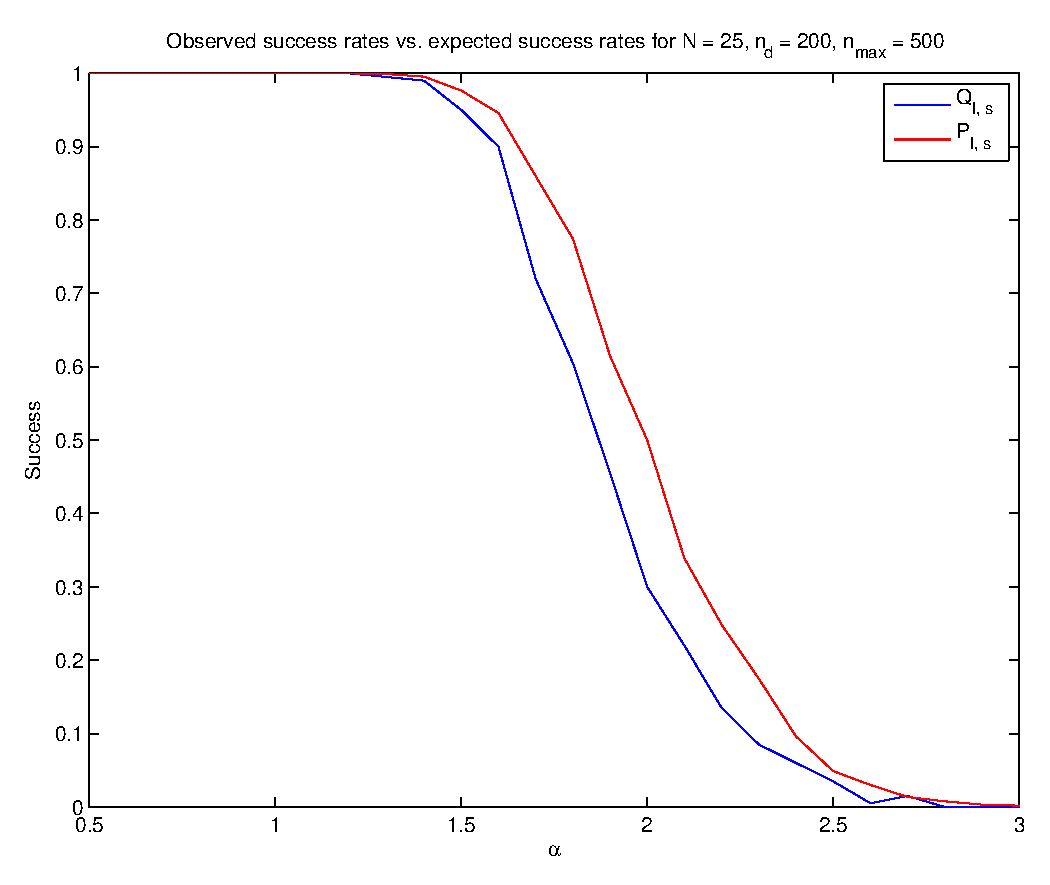
\includegraphics[width=\columnwidth]{success_rate_N_25_nd_200_nmax_500.eps}%
	\figcaption{The observed success rate (shown in blue) descends as \(\alpha\) increases.}
	\label{fig:25neurons}
}
Figure~\ref{fig:25neurons} plots the observed success rate versus the expected success rate for 25 neurons.
It is clear that as \(\alpha\) increases, the fraction of successful trainings decreases.
\myfigure{
	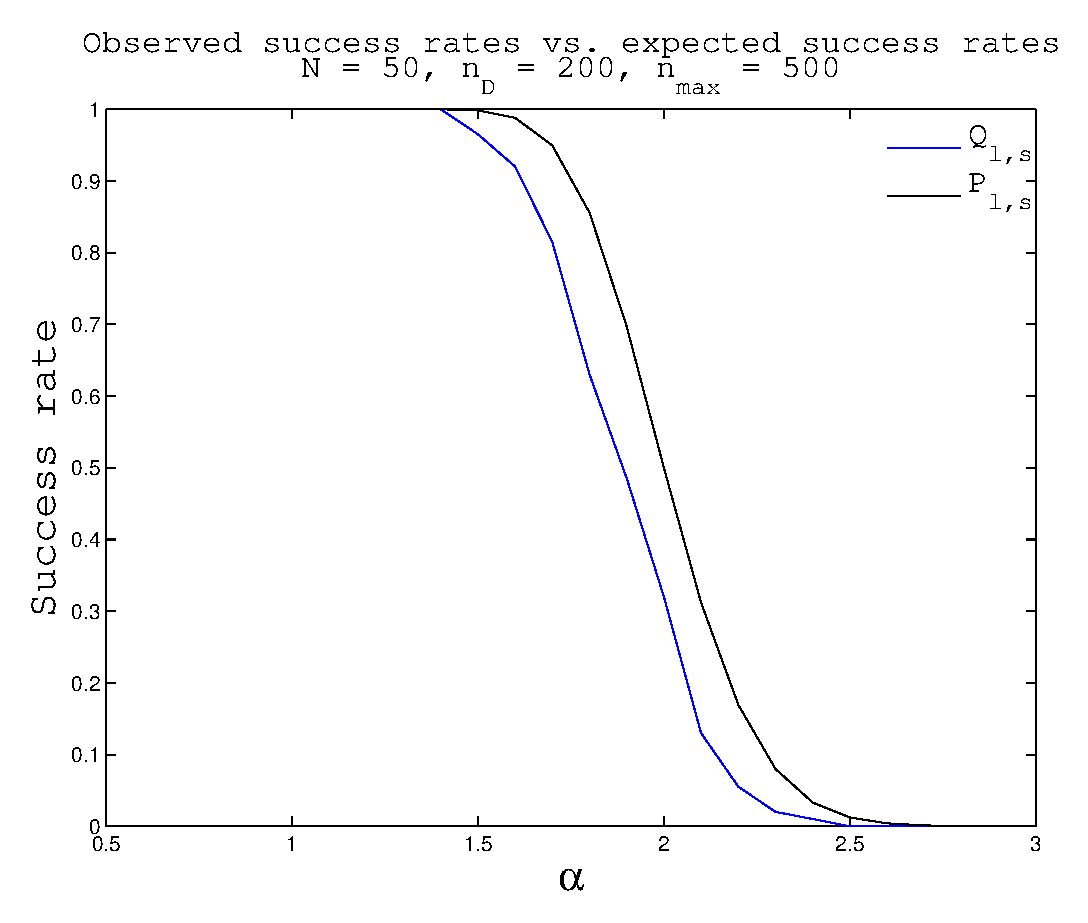
\includegraphics[width=\columnwidth]{success_rate_N_50_nd_200_nmax_500.eps}%
	\figcaption{The observed success rate (shown in blue) descends faster as \(\alpha\) increases.}
	\label{fig:50neurons}
}
Using 50 neurons as opposed to 25 neurons yields an interesting observation:
The success rate descends faster, in a smaller interval in \(\alpha\).
\myfigure{
	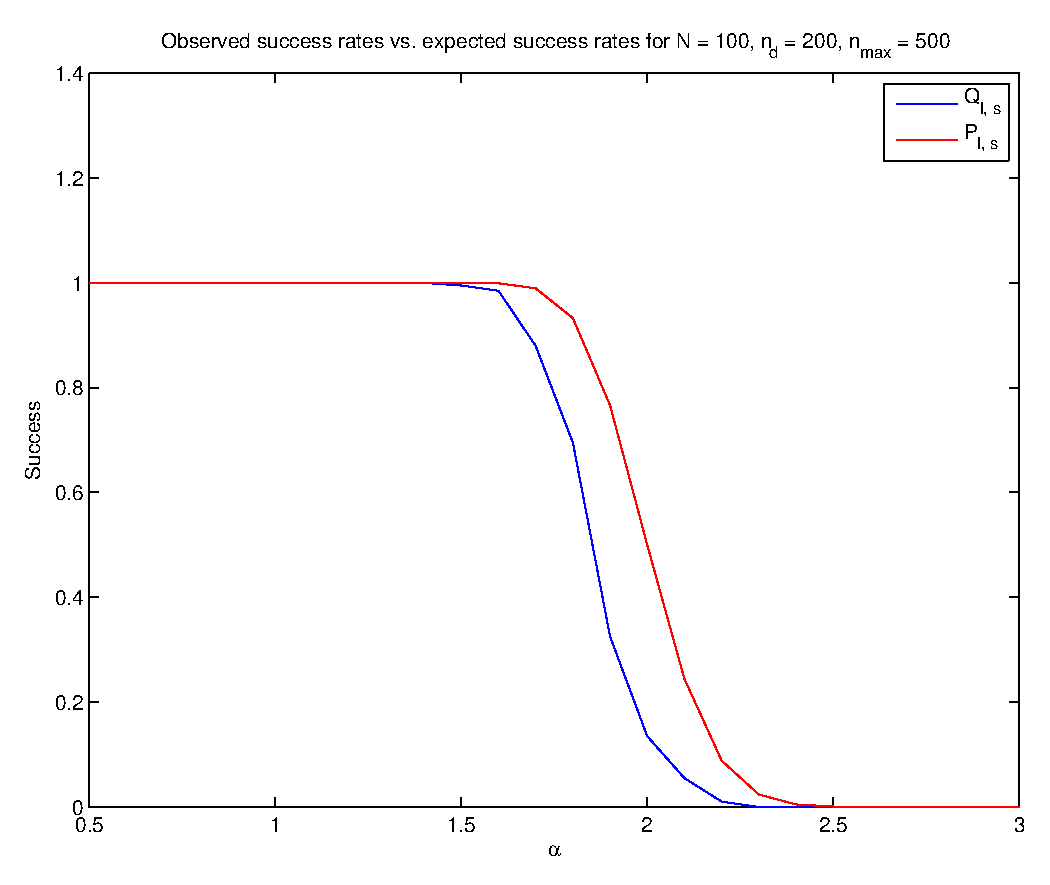
\includegraphics[width=\columnwidth]{success_rate_N_100_nd_200_nmax_500.eps}%
	\figcaption{The observed success rate (shown in blue) descends rapidly as \(\alpha\) increases.}
	\label{fig:100neurons}
}

When 100 neurons are used, the success rate descends even faster, and starts to resemble the step function with the step around \(\alpha = 1.75\).
